\documentclass[12pt, a4paper, openany]{report}
\def\VersionRapport{1.0}
\usepackage[utf8]{inputenc} % un package
\usepackage[T1]{fontenc}      % un second package
\usepackage[francais]{babel}  % un troisième package
\usepackage{layout}
\usepackage[top=2.7cm, bottom=2.5cm, left=3.5cm, right=3cm]{geometry}
\usepackage{setspace}
\frenchbsetup{StandardLists=true} % à inclure si on utilise \usepackage[french]{babel}
%\usepackage{enumitem}
\usepackage[shortlabels]{enumitem}
\usepackage{amssymb}
\usepackage{color}
\usepackage{listings}
\definecolor{dkgreen}{rgb}{0,0.6,0}
\definecolor{gray}{rgb}{0.5,0.5,0.5}
\definecolor{mauve}{rgb}{0.58,0,0.82}
\definecolor{rougecerise}{rgb}{0.73,0.043,0.043}
\lstset{frame=tb,
  language=Matlab,
  aboveskip=3mm,
  belowskip=3mm,
  showstringspaces=false,
  columns=flexible,
  basicstyle={\small\ttfamily},
  keywordstyle=\color{blue},
  commentstyle=\color{dkgreen},
  stringstyle=\color{mauve},
  breaklines=true,
  breakatwhitespace=true,
  tabsize=3,
  breaklines=true,
  morekeywords={matlab2tikz},
  morekeywords=[2]{1}, 
  keywordstyle=[2]{\color{black}},
  identifierstyle=\color{black},
  numbers=left,
  numberstyle={\tiny \color{black}},
  numbersep=9pt, 
  emph=[1]{for,end,break},
  emphstyle=[1]\color{red}
}
\usepackage{multirow} % pour les tableaux
\usepackage[table]{xcolor} % pour les tableaux
\usepackage{verbatim}
%\usepackage{subcaption}
\usepackage{graphicx}
\usepackage{moreverb}
\usepackage{url}
\usepackage{pst-all}
\usepackage{eso-pic,graphicx}
\usepackage{caption} 
\usepackage[colorlinks=true,urlcolor=blue,linkcolor=red]{hyperref}
\usepackage{array}
\usepackage[toc,page]{appendix}
\usepackage[off]{auto-pst-pdf}
\usepackage{hyperref} % pour le sommaire table des matières
\AddThinSpaceBeforeFootnotes % à insérer si on utilise \usepackage[french]{babel}
\FrenchFootnotes % à insérer si on utilise \usepackage[french]{babel}
\usepackage{fancyhdr}
\pagestyle{headings}
\usepackage{pifont}  %pour les puces
\usepackage{amsmath} %pour les puces
\usepackage{subfig}
\usepackage{verbatim} % pour le code en annexe 
%%%%%%%colones 
\newcolumntype{R}[1]{>{\raggedleft\arraybackslash }b{#1}}
\newcolumntype{L}[1]{>{\raggedright\arraybackslash }b{#1}}
\newcolumntype{C}[1]{>{\centering\arraybackslash }b{#1}}
%%%%%%% 
\renewcommand{\appendixpagename}{Annexes}
\renewcommand{\appendixtocname}{Annexes}
\title{Theme: Compte Rendu SLI 2}
\author{TEVENINO \bsc{Namataiki} \\ KHERBICHE \bsc{Ali}}
\date{2018-2019}
%new
\newcommand{\HRule}{\rule{\linewidth}{0.5mm}}

\begin{document}

%\selectlanguage{francais}
\pagenumbering{arabic} 
\makeatletter
\begin{titlepage}
\begin{sffamily}
\begin{center}
    % Upper part of the page. The '~' is needed because \\
    % only works if a paragraph has started.
    
\includegraphics[scale=0.5]{Logo_UT3.jpg}~\\[1cm]
    \textsc{\LARGE M1 ISTR-RODECO  }\\[1cm]
    \textsc{\Large Compte Rendu SLI 2}\\[1cm]
    % Title
    \HRule \\[0.4cm] % saut de ligne
    { \huge  \textsc {Synthèse d'un asservissement de position par retour d'état continu avec observateur \\[0.4cm] }}

    \HRule \\[1cm]   % sous de ligne 
    
\includegraphics[scale=0.1]{logomaster.jpg}
    \\[1cm]
    % Author and supervisor
    \begin{minipage}{0.4\textwidth}
      \begin{flushleft} \large
         \textsc{\emph {Fait par:} \\KHERBICHE Ali\\ TEVENINO Namataiki}  
          \newline
          Promotion 2018-2019 \\
      \end{flushleft}
    \end{minipage}
    \begin{minipage}{0.4\textwidth}
      \begin{flushright} \large
        %%\emph{Tuteur et}
        \emph{Tuteurs:} \textsc{M.Frédéric GOUAISBAUT\\M.Sylvain DUROLA}
      \end{flushright}
    \end{minipage}
    \vfill
    % Bottom of the page
    {\large Décembre 2018}
  \end{center}
  \end{sffamily}                
  \end{titlepage}  
\makeatother
   
%*********************** somaire **************
\renewcommand{\contentsname}{Sommaire}
\tableofcontents
%*********************** listes des figures **************
\listoffigures
%*********************** listes des tableaux **************
%\listoftables

\chapter*{\textsc{Introduction}}
\addcontentsline{toc}{chapter}{\textsc{Introduction}}
	
	\paragraph{}
		Cette manipulation se propose de réaliser un asservissement de position en mettant en œuvre les techniques d’espace d’état continu. Le procédé utilisé est la platine ”asservissement de position" qui apparaît dans la \hyperref[fig1]{Figure 1}, déjà présentée dans les textes des manipulations des TP de licence EEA (2ème année) dont le principe est rappelé sur le schéma présenté dans la \hyperref[fig2]{Figure 2.}

	\begin{center}
	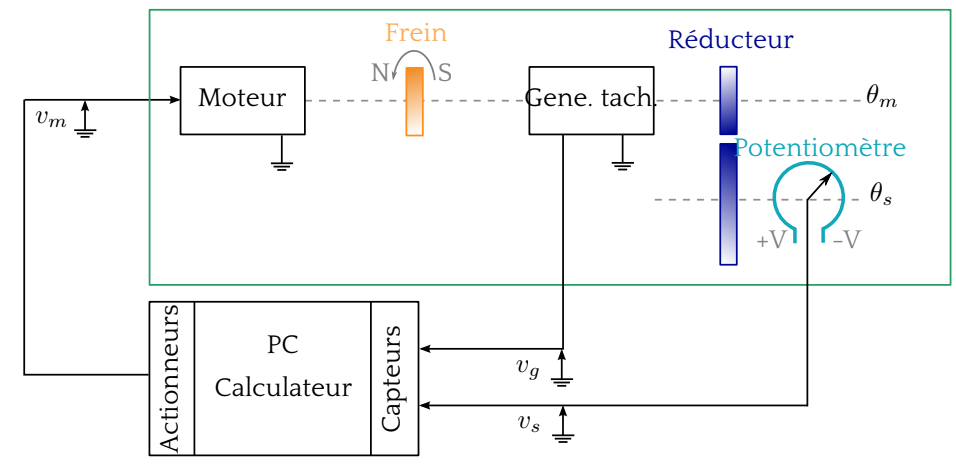
\includegraphics[scale=0.4]{schemamotor.png}
	\captionof{figure}{\textit{Asservissement de position par calculateur\\}}
	\label{fig1} 
	\end{center} 
	
	\begin{center}
	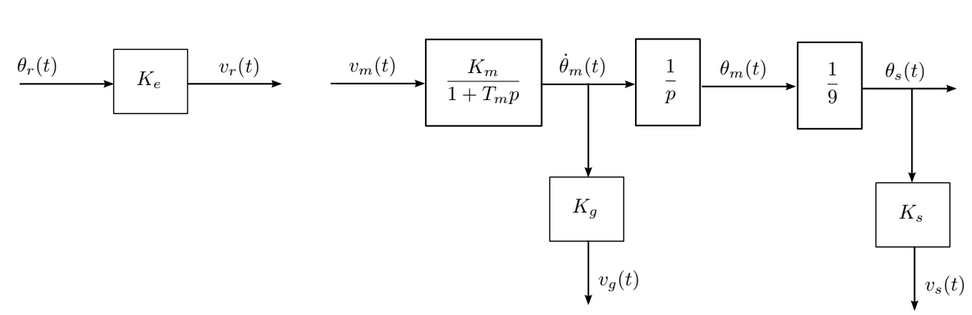
\includegraphics[scale=0.4]{schemablocmotor.png}
	\captionof{figure}{\textit{Eléments de la platine (asservissement de position)\\[4cm]}}
	\label{fig2} 
	\end{center}
	
	\begin{itemize} [label=\ding{70},font=\small \color{black}]
	\item $v_{m}(t)$\hspace{1mm} est la tension d'entrée du moteur.
	\item $\theta_{s}(t)$\hspace{1mm} est la position de l'axe secondaire du moteur.
	\item $\dot{\theta}_{m}(t)$ est la vitesse de rotation de l'axe principal du moteur.\\
	%Les paramètres $K_{m}$ et $\tau_{m}$ ont déjà été déterminés lors du TP2 de SLI1. 
	Les coefficients connus sont $K_{e}$, $K_{s}$ et $K_{g}$, leurs valeurs numériques sont données comme suit:
	\begin{itemize} [label=\ding{171},font=\small \color{black}]
	\item $K_{e} = 10(V.tr^{-1})$
	\item $K_{s} = 10(V.tr^{-1})$
	\item $K_{g} = 0.105(V.s.tr^{-1})$
	%\item $K_{m} = 10$
	%\item $K_{g} = 0.29(s)$
	\end{itemize}
	\end{itemize}
	
	\paragraph{}
		Il est possible d’obtenir une mesure de $\theta_{s}(t)$ et de $\theta_{m}(t)$ via un potentiomètre et une génératrice tachymétrique.
		
		\begin{center}
		$v_{m}(t) = K_{s}\theta_{s}(t)$ \hspace{1.5cm} et \hspace{1.5cm} $v_{g}(t) = K_{g}\dot{\theta}_{m}(t)$ 
		\end{center}
		

\chapter{\textsc{Identification et analyse du procédé}}
\addcontentsline{toc}{chapter}{\textsc{Identification et analyse du procédé}}


\section{\textsc{Identification des coefficients $K_m$ et $T_m$}}

\par Grâce à un oscilloscope, on obtient des signaux comme montré sur la figure ci-desous :

\begin{figure}[h!]
\centering
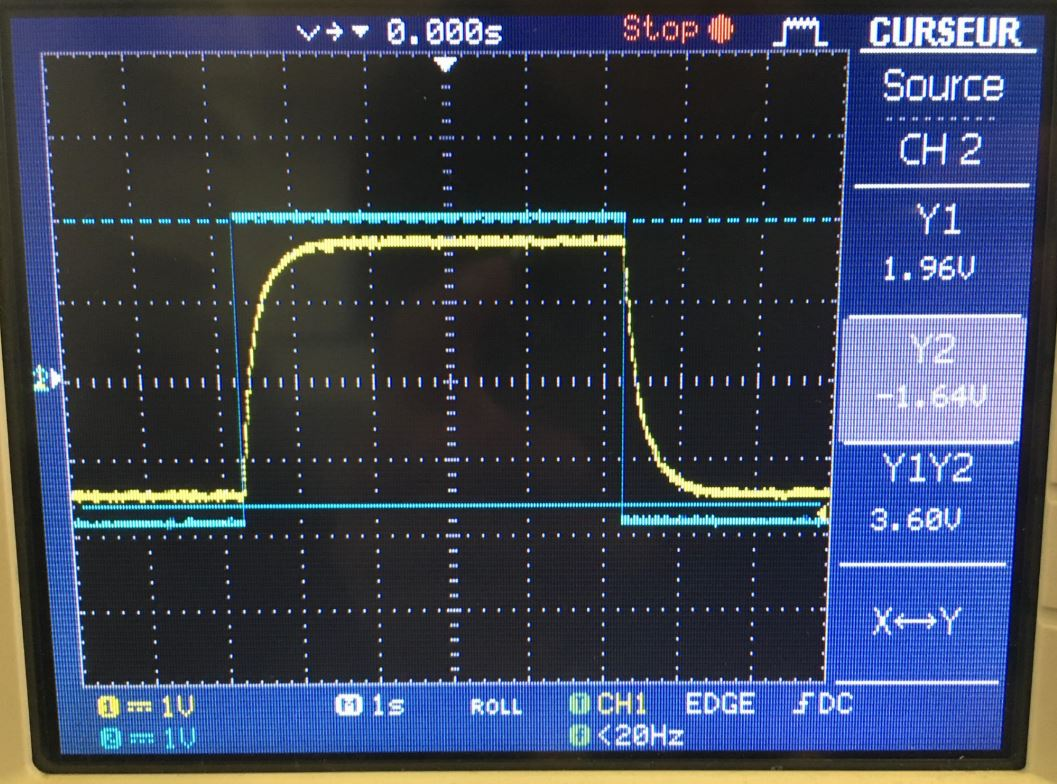
\includegraphics[scale = 0.5]{trace_temp_syst.JPG}\\[1 cm] 
\caption{Tracé temporelle du système}
\end{figure}

\par Tout d'abord nous avons mesurés le temps de monté du signal à $t_m=130ms=0.13sec$ à l'aide des curseurs (90 pour cent de la valeur finale). Afin de trouver $T_m$ nous avons utilisé une relation définit par $T_m=3*\tau$. \\

\par Or $\tau=\frac{0.13*63}{100}=0.0819sec$. Donc \fbox{$T_m=3*\tau=0.26$}\\

\par Ensuite nous avons mesuré le gain aporté sur le signal, $gain=\frac{Y_2}{Y_1}=0.837$. Or d'après le schéma de la figure 2, on a $gain=K_gK_m$ et $K_g=0.105$. Donc \fbox{$K_m=\frac{gain}{K_g}=\frac{0.837}{0.105}=8$} \\

\par Nous avons donc trouvé expérimentalement le gain en vitesse $K_m = 8$ et la constante de temps mécanique $T_m=0.26$.\\


\section{\textsc{Représentation et analyse de l'ensemble pour le système $S_{v_m->v_s}$}}

\paragraph{} On considère le système en boucle ouverte $S_{v_m->v_s}$, qui admet comme entrée le signal $v_m(t)$ et comme sortie le signal mesurée $v_s(t)$. En fonction de nos variables et de nos coefficients décrit précédement, nous avons définit la représentation d'état de ce système, en choisissant un vecteur d'état défini par :\\
$$x(t)=[x_1(t)~~x_2(t)]^T=[v_s(t)~~v_g(t)]^T$$

\paragraph{} D'après le schéma on a : $v_s(t)=K_s\theta_s(t)$ et $v_g(t)=K_g\dot{\theta_m}(t)$\\

\par Donc : $x_1(t)=K_s\theta_s(t)$ et $x_2(t)=K_g\dot{\theta_m}(t)$\\

\par Grâce a la relation sortie sur entrée on obtient : \Large$\frac{v_s(p)}{v_m(p)}=\frac{K_sK_m}{9p(1+T_mp)}$\\

\par \normalsize D'où : \Large$x_1(p)=\frac{K_sK_m}{9p(1+T_mp)}v_m$\\

\par \normalsize Or : \Large$\dot{\theta_m}(p)=\frac{K_m}{1+T_mp}v_m=\frac{v_g}{K_g}$\\

\par \normalsize On a donc : \Large$x_1=\frac{K_sv_g}{9pK_g}$\\

\par \normalsize D'où : \Large\fbox{$\dot{x_1}=\frac{K_s}{9K_g}v_g$}\\

\par \normalsize A partir de $v_g$ on trouve $\dot{x_2}$ : \Large$v_g=\frac{K_gK_mv_m}{1+T_mp}$\\

\par \normalsize On transforme $v_g$, ce qui donne : \Large$v_g=\frac{K_mK_g}{T_m}\frac{T_m}{T_mp+1}v_m$=$\frac{K_mK_g}{T_m}\frac{1}{p+\frac{1}{T_m}}v_m$\\

\par \normalsize D'où : \Large$v_g(p+\frac{1}{T_m})=\frac{K_mK_g}{T_m}v_m$\\

\par \normalsize On obtient donc : \Large$v_gp=\dot{v_g}$=\fbox{$\dot{x_2}=\frac{K_mK_g}{T_m}v_m-\frac{1}{T_m}v_g$}\\

\par \normalsize La représentation d'état du système ce présente comme ceci :\large
$$\dot{x}=\begin{bmatrix}\dot{x_1}\\\dot{x_2}\end{bmatrix}=\begin{bmatrix}0 && \frac{K_s}{9K_g} \\ 0 && -\frac{1}{T_m}\end{bmatrix}\begin{bmatrix}x_1\\x_2\end{bmatrix}+\begin{bmatrix}0\\\frac{K_mK_g}{T_m}\end{bmatrix}V_m$$
$$y=\begin{bmatrix}1&&0\end{bmatrix}x+0$$\\

\par \normalsize Par identification on obtient nos matrices:
$$A=\large\begin{bmatrix}0&&\frac{K_s}{9K_g}\\0&&-\frac{1}{T_m}\end{bmatrix} ; \normalsize B=\large\begin{bmatrix}0&&\frac{K_mK_g}{T_m}\end{bmatrix} ; \normalsize C=\large\begin{bmatrix}1&&0\end{bmatrix} ; \normalsize D=\large0$$\\

\par On obtient numériquement, si $T_m=0.3$ et $K_m=7$ :
$$A=\begin{bmatrix}0&&10.6\\0&&-3.33\end{bmatrix} ; \normalsize B=\begin{bmatrix}0&&2.45\end{bmatrix} ; \normalsize C=\begin{bmatrix}1&&0\end{bmatrix} ; \normalsize D=0$$
~~\\

\par Nous supposons que $v_m$=0, cela veut dire qu'il n'y aurait auncune puissance en entrée de notre système. Donc le système ne fonctionnerais pas et sera immédiatement aux points d'équilibre. C'est à dire $v_{se}(t)=0$ et $v_{ge}(t)=0$.\\

\par Supposons maintenant que $v_m=v_{m0}=constante$. Le système sera donc constamment en mouvement, donc en fonctionnement. Et n'atteindra jamais une position aux points d'équilibre.\\

\par Nous avons deux façon de déterminer si le système $S_{v_m->v_s}$ est stable ou instable, cela se fait évidemment autours des points de fonctionnement. Pour la première méthode, nous avons vu en cours que la fonction de transfert s'écrit d cette manière : \large $$PI=C(\lambda I-A)^{-1}B+D$$ \normalsize \\

\par Après transformation avec nos variables des matrices, on obtient ceci : 
\large$FT=\frac{1}{p^2+\frac{1}{T_m}p}\frac{K_sK_m}{9T_m}$ \normalsize \\

\par Par la suite nous étudions les pôles de cette fonction de transfert (le dénominateur) :
\large$p^2+p\frac{1}{T_m}=0~~<=>~~p(p+\frac{1}{T_m})=0$ \normalsize \\

\par Nous avons ici deux solutions, $p=0$ ou $p=-\frac{1}{T_m}$. On conclu dontème est instable, car on a un pôle positif (Instable si un pôle $\ge0$).\\

\par Pour la deuxième méthode, on cherche tout d'abord le "det$(\lambda I-A)$" et on calcule les $\lambda_1$ et $
\lambda_2$. Si la partie réel des $\lambda_1$ et $\lambda_2$ est négatif, alors le système est instable :
$$det(\large\begin{bmatrix}\lambda && 0 \\ 0 && \lambda \end{bmatrix} - \begin{bmatrix}0 && \frac{K_s}{9K_g} \\ 0 && -\frac{1}{T_m}\end{bmatrix}\normalsize)=0$$ \\

\par Ce qui donne : $$det\large\begin{bmatrix}\lambda && 0-\frac{K_s}{9K_g} \\ 0 && \lambda-\frac{K_s}{9K_g} \end{bmatrix}\normalsize=0$$ \\

\par Puis :
$$\lambda(\lambda-\frac{K_s}{9K_g})=0$$ \\

\par On a donc :
$$\lambda_1=0~~;~~\lambda_2=-\frac{1}{T_m}$$ \\

\par On peut donc conclure également que le système est instable.\\

\par On remarque que le système $S_{v_m->v_s}$ présente deux modes. Le mode stationnaire ($\lambda_1=0$) et le mode convergent ($\lambda_2=-\frac{1}{T_m}$).\\

\section{\textsc{Commandabilité et observabilité}}

\par Intéressons nous à la commandabilité ainsi qu'à l'observabilité du sytème $S_{v_m->v_s}$. Comme d'écrit dans l'énoncé, on a un vecteur d'état avec deux variables d'état : $$x(t)=\begin{bmatrix}x_1(t)&&x_2(t)\end{bmatrix}^T$$\\

\par On peut donc écrire : $Com=\begin{bmatrix}A&&AB\end{bmatrix}$ et $Obs=\begin{bmatrix}C\\CA\end{bmatrix}$ \\

\par D'où: $$Com = \begin{bmatrix}0&&25.7\\2.47&&0\end{bmatrix}$$\\
$$Obs = \begin{bmatrix}1&&0\\0&&10.5\end{bmatrix}$$\\

\par Aucune combinaison n'est possible afin de trouver une égalité entre colonnes ou lignes des deux matrices Observable et Commandable, ils sont tous les deux de rang 2 (= nombres de variables d'état). On peut donc en conclure que le système est commandable et observable également \label{section 1.2} \hyperref[Annexe A]{voir Annexe A.}\\

%\par Etant donné que notre système a un couple (A,B) commandable, donc il admet une représentation compagne de commande. Idem pour le couple (A,C) observable, notre système admet donc une représentation compagne d'observation.\\

%\section{\textsc{Représentation et analyse de l'ensemble pour le système $S_{v_m->v_g}$}}
%\par On considère ici le système en boucle ouverte $S_{v_m->v_g}$, qui admet comme entrée le signal $v_m(t)$ et comme sortie le signal mesurée $v_g(t)$. On avait 
%$$v_s=y=\begin{bmatrix}1&&0\end{bmatrix}\begin{bmatrix}v_s\\v_g\end{bmatrix}+0~U_m$$
%\par Avec cette sortie on a $v_g=0$. Or ici on veut en fonction de $v_g$ (car on étudie sur le système $S_{v_m->v_g}$). Donc seul la matrice C change, et l'espace d'état dynamique d'entré $\dot{x}(t)$ ne change pas : $$C=\begin{bmatrix}0&&1\end{bmatrix}$$\\
%~~\\
%\par Afin d'étudier la stabilité du système nous avons uniquement besoin de la matrice A, et calculer le déterminant de $(\lambda I-A)$. Or la matrice A n'a pas changé, et ce déterminant a déjà été calculé précédement. Les propriétés de stabilité du système $S_{v_m->v_g}$ reste identique à celles du système $S_{v_m->v_s}$. Le nouveau système considéré est donc stable.\\
%~~\\
%\par De même, le nouveau système considéré est commandable. Car le couple de commande (A,B) est toujours de rang 2. Cependant on ne peut pas en dire pareil pour son observabilité :
%$$Obs=\begin{bmatrix}C\\CA\end{bmatrix}=\begin{bmatrix}0&&1\\0&&-\frac{10}{3}\end{bmatrix}$$
%\par On remarque ici que cette matrice est de rang 1. Elle n'est donc pas observable, car il existe une combinaison permettant de passer d'une colonne à l'autre $->$ fois 0 (idem pour les lignes).
%\par Ce résultat était prévisible car la matrice C a changé et qu'on a une colonne nulle.
%
%\pagebreak

\chapter{\textsc{Mise en place d'un retour d'état}}
\addcontentsline{toc}{chapter}{\textsc{Mise en place d'un retour d'état}}

	\section{\textsc{Annulation de l'erreur de position}}
	
	\par Pour un système SISO (une entrée/une sortie) les pôles permettent de régler la dynamique du système, c’est-à-dire, le régime transitoire. Par contre, cette technique ne permet pas de régler le problème de la précision. Nous ne pouvons pas choisir le régime permanent du système en boucle fermée par le choix de K. Nous proposons une première structure de commande permettant d’assurer une erreur de position nulle en régime permanent tel que \cite{ref1} :
	
	\begin{center}
	$u(t) = -Kx(t) + Ny_{ref}(t)$ 
	\end{center}		

	Où le pré-compensateur $N$ est un gain matriciel permettant de régler le gain statique du système en boucle fermée, avec:
	
	\begin{center}
	$N = \frac{1}{C(BK-A)^{-1}B}$ 
	\end{center}	
%\par Avec MATLAB\label{section 3.3} \hyperref[Annexe A]{voir Annexe A}, on a trouvé: $N= 1.389$.

	\section{ \textsc{Calcul des paramètres du retour d'état $K$ et $N$}}
	
\par Ce système est réalisé selon la loi de commande par retour d'état $v_m(t)=NK_e\theta_r(t)-Kx(t)=Nv_r(t)-Kx(t)$, avec $K=\begin{bmatrix}k_1 && k_2\end{bmatrix}$\\
\par Nous avons déterminé l'expression du modèle du système asservi par le retour d'état mentionné plus haut en fonction de K et N. On a tout d'abord :\\
~~\\
$\dot{x}=Ax+Bv_m \\ y=Cx+Dv_m$\\
\par On remplace $v_m$ :\\
$\dot{x}=Ax+B[Nv_r-Kx] \\ y=Cx+D[Nv_r-Kx]$\\
\par On distribue :\\
$\dot{x}=Ax+BNv_r-BKx \\ y=Cx+DNv_r-DKx$\\
\par Et on factorise :\\
$\dot{x}=(A-BK)x+BNv_r \\ y=(C-DK)x+DNv_r$\\
\par Ce qui nous donne comme expression de nos matrice :\\
$$A_{bf}=\begin{bmatrix}A-BF\end{bmatrix} ; B_{bf}=\begin{bmatrix}BN\end{bmatrix} ; C_{bf}=\begin{bmatrix}C-DF\end{bmatrix} ; D_{bf}=0$$
\par En remplaçant A, B et F dans la matrice $A_{bf}$, cela nous donne :
$$A_{bf}=A_{bf}=\begin{bmatrix}0 && \frac{K_s}{9K_g} \\ 0 && -\frac{1}{T_m}\end{bmatrix}-\begin{bmatrix}0 \\ \frac{K_mK_g}{T_m}\end{bmatrix}\begin{bmatrix}k_1 && k_2\end{bmatrix}$$
\par D'où $$A_{bf}=\begin{bmatrix}0 && \frac{K_s}{9K_g} \\ -\frac{K_mK_gk_1}{T_m} && -\frac{1}{T_m}-\frac{K_gK_mk_2}{T_m}\end{bmatrix}$$\\
\par Comme nous avons vu précédement, le système $S_{v_m->v_s}$ est commandable en (A,B). On peut donc placer les valeurs propres de la matrice $A_{bf}$ en $v_1$ et $v_2$.
\par Nous avons ensuite chercher la valeur de K, tel que les valeurs propres du système asservi soient $v_1$ et $v_2$. On sait que : det$(\lambda I-A{bf})$=$(p-v_1)(p-v_2)$. Nous avons donc d'abord chercher le detéminant :
$$det(\begin{bmatrix}\lambda && 0 \\ 0 && \lambda\end{bmatrix}-\begin{bmatrix}0 && \frac{K_s}{9K_g} \\ -\frac{K_gK_mk_1}{T_m} && -\frac{1}{T_m}-\frac{K_gK_mk_2}{T_m}\end{bmatrix})=det \begin{bmatrix}\lambda && -\frac{K_s}{9K_g} \\ -\frac{K_gK_mk_1}{T_m} && \lambda+\frac{1}{T_m}+\frac{K_gK_mk_2}{T_m}\end{bmatrix}$$
\par Ce qui nous donne :
$$\lambda^2+[\lambda(\frac{1+K_gK_mk_2}{T_m})]-[\frac{K_gK_mk_2}{T_m}\frac{-K_s}{9K_g}]$$
\par Après développement on a :
$$\lambda^2+\frac{1}{T_m}\lambda+\frac{K_gK_mk_2}{T_m}\lambda+\frac{K_mK_sk_1}{9T_m}$$
%\par On simplifie et on numérise, c'est à dire on remplace par leurs valeurs :
%$$\lambda^2+(\frac{1}{0.26}+\frac{0.105*8}{0.26}k_2)\lambda+\frac{8*10}{9*0.26}k_1=(p-v_1)(p-v_2)$$
\par On a aussi : 
$$(\lambda-v_1)(\lambda-v_2)=(\lambda+2.4-5.5j)(\lambda+2.4+5.5j)$$
%\par Ce qui donne :
%$$p^2+2.4p+5.5jp+2.4p+5.76+13.2j-5.5jp-13.2j+30.25=p^2+4.8p+36.01$$
\par On identifie ensuite avec l'équation du déterminant,\label{K} \hyperref[annexe B]{Voir annexe B :}\\

\begin{center}

\fbox{$K=\begin{bmatrix}k_1&&k_2\end{bmatrix}=\begin{bmatrix}1.0533&&0.2362\end{bmatrix}$}

\end{center}

\par Ensuite il ne reste qu'à déterminer la valeur du pré-compensteur $N$, \label{N} \hyperref[Annexe C]{Voir annexe C :}
\begin{center}

\fbox{$N= 1.0533$}

\end{center}


\chapter{\textsc{Compensation par retour de sortie dynamique - observateur fonctionnel}}
\addcontentsline{toc}{chapter}{\textsc{Compensation par retour de sortie dynamique - observateur fonctionnel}}
\chaptermark{\textsc{Compensation par retour de sortie dynamique - observateur fonctionnel}}
\section{\textsc{Observateur identité}}
\par Dans cette partie on veut construire un observateur identité à partir de l'entrée $v_m(t)$ et de la tension de sortie $v_s(t)=K_s\theta_s(t)$, mais également que l'observateur soit 2 fois, 4 fois puis 8 fois plus rapide que la dynamique de la boucle fermée.
\par On veut donc obtenir un système de cette forme :\\
~~\\
$\widehat{x}(t) = Mz(t) + Dy(t)$\\
$\dot{z}(t) = Fz(t)Gy(t) + Hu(t))$
\par Avec : H = B ; M = $I_{2}$ et D = 0.
\par On pose : $$F = \begin{bmatrix}f_{11} && f_{12} \\ f_{21} && f_{22} \end{bmatrix}~~~~et~~~~G = \begin{bmatrix}g_1 \\ g_2 \end{bmatrix}$$
\par Cela nous donne : 
$$F =  \begin{bmatrix}f_{11} && f_{12} \\ f_{21} && f_{22} \end{bmatrix} = \begin{bmatrix}0 && 10.5820 \\0 && -3.33 \end{bmatrix} - \begin{bmatrix}g_1 \\ g_2 \end{bmatrix}*\begin{bmatrix}1 && 0 \end{bmatrix}$$
\par A l'aide de Mathlab et la fonction "acker", nous avons calculé la matrice G et F :\\
~~\\
$P=[-2.4+5.5*i -2.4-5.5*i]\\
~~\\
G=acker(A’,C’,P)’\\
G1=acker(A’,C’,2*P)’\\
G2=acker(A’,C’,4*P)’\\
G3=acker(A’,C’,8*P)’\\
~~\\
F=A-G*C\\
F1=A-G1*C\\
F2=A-G2*C\\
F3=A-G3*C$


\paragraph{} D'où : $ F = \begin{bmatrix} -1.4667 && 10.5820 \\ -2.9409 && -3.3333 \end{bmatrix} $ et $ G = \begin{bmatrix}1.4667 \\ 2.9409\end{bmatrix} $\\
\par Par la suite, nous avons modélisé ce système à l'aide de Simulink notre schéma bloc, qui se présente de cette façon :
\begin{figure}[h!]
\centering
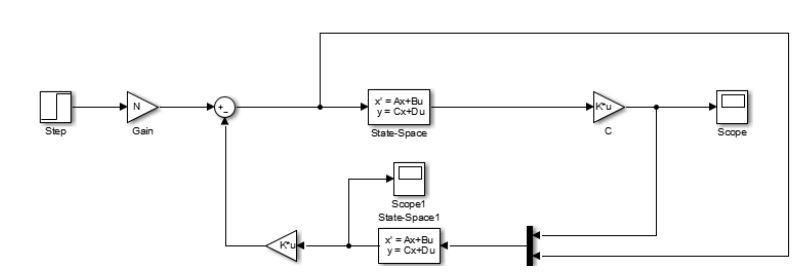
\includegraphics[scale = 0.7]{SIM1.JPG}\\[0.7 cm] 
\caption{Schéma bloc de l'observateur identité}
\end{figure}
\par La simulation donne donc :
\begin{figure}[h!]
\centering
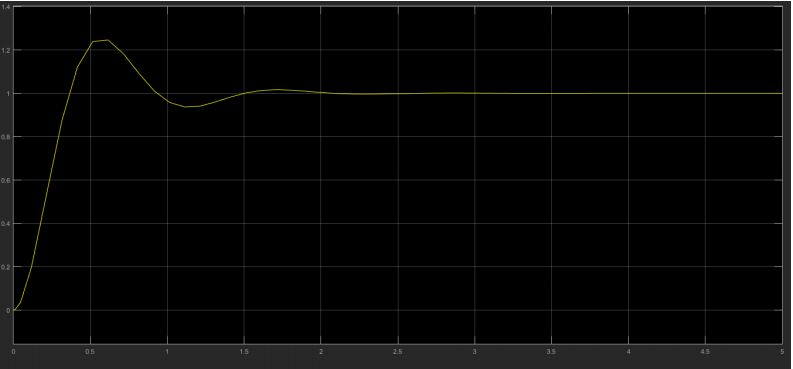
\includegraphics[scale = 0.7]{T1.JPG}\\[0.7 cm] 
\caption{Simulation observateur identité}
\end{figure}
\par On peut observer que le signal converge bien vers 1, qui est la consigne.
\par Ici nous avons calculé les gain de l'observateur de manière à modifier ses valeur propres pour que l'observateur soit d'abors 2 fois, puis 4 fois et enfin 8 fois plus rapide que la dynamique de la boucle fermée.
\par Pour cela nous avons multiplié par le nombre de fois qu'on veut les valeurs propres. Nous obtenon donc ceci :
$$F1 = \begin{bmatrix}-6.2667 && 10.5820 \\ -11.6378 && -3.3333\end{bmatrix}~~~~et~~~~G1 = \begin{bmatrix}6.2667 \\ 11.6378\end{bmatrix}$$
$$F2 = \begin{bmatrix}-15.8667 && 10.5820 \\ -49.4491 && -3.3333\end{bmatrix}~~~~et~~~~G2 = \begin{bmatrix}15.8667 \\ 49.4491\end{bmatrix}$$
$$F3 = \begin{bmatrix}-35.0667 && 10.5820 \\ -206.7425 && -3.3333\end{bmatrix}~~~~et~~~~G3 = \begin{bmatrix}35.0667 \\ 206.7425\end{bmatrix}$$
\par Nous avons ensuite modélisé trois observateur pour nos trois rapidité par des schéma bloc sur Simulink, comme montré ci-dessous :
\begin{figure}[h!]
\centering
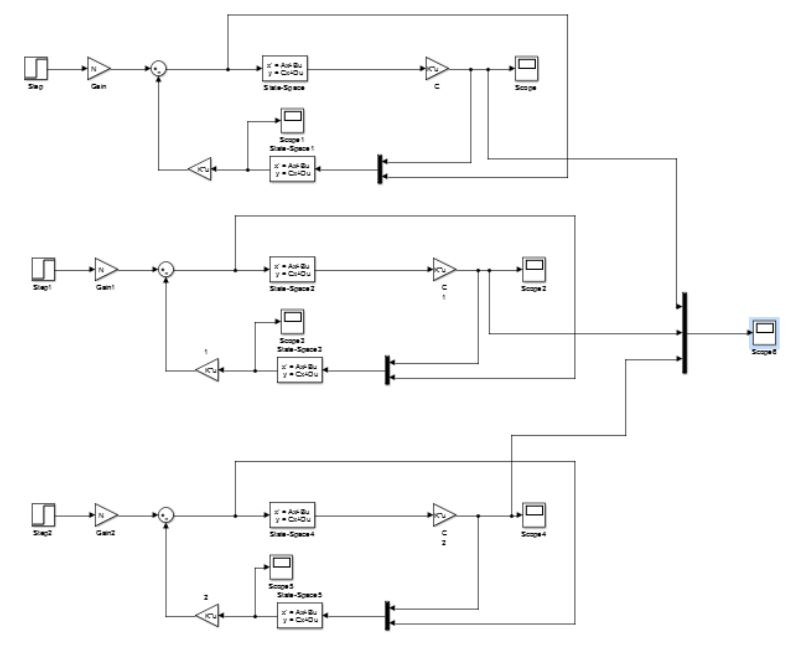
\includegraphics[scale = 0.7]{3OBS.JPG}\\[0.7 cm] 
\caption{Schéma bloc de trois observateurs}
\end{figure}
\pagebreak
\par Les tracés aux conditions initiales $v_s(0)=\pi/2~et~\dot{v_s}(0)=0$ nous donne évidemment trois courbes, qui sont de cette forme :
\begin{figure}[h!]
\centering
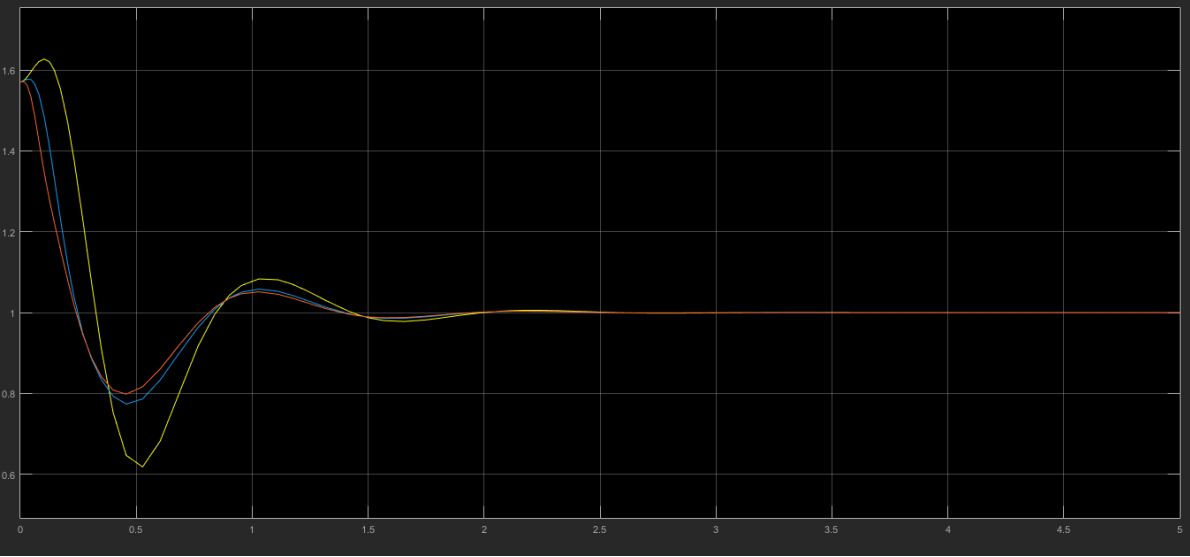
\includegraphics[scale = 0.45]{T_3OBS.JPG}\\[0.7 cm] 
\caption{Sortie des trois observateurs}
\end{figure}
\par On peut conclure que plus on augmente la valeur des valeurs propres et plus le système sera rapide d'où une convergence plus rapide des la sortie. De plus on observe une minime diminution du dépassement lorsque les valeurs propres augmentent.

\section{\textsc{Observateur minimal identité}}
\par Dans cette partie on veut construire un observateur minimal identité à partir de l'entrée $v_m(t)$ et de la tension de sortie $v_s(t)=K_s\theta_s(t)$, mais également que l'observateur sois 4 fois plus rapide que la dynamique de la boucle fermée.
\par On a notre matrice A, que l'on peut écrire de cette façon :
    $$A = \begin{bmatrix}0 && 10.5820 \\0 && -3.33 \end{bmatrix}$$
\par $A_{11}=0~; A_{12}=10.5820~; A_{21}=0~; A_{22}=3.33$
\par Et $B_1 = 0~~et~~B_2 = 3.5$
\par Dans cette partie notre nouveau système s'écrit de cette manière :\\
~~\\
$\dot{s}(t) = F_1s(t) + G_{tild}y(t)+H_{tild}u(t)$\\
$\widehat{z}(t) = s(t) + G_1y(t))$
\par On sait que :
$$G_{tild} = F_1G_1 - G_1A_{11} + A_{21}$$
$$H_{tild} = B_2G - GB_1$$
$$F_1=A_{22} - G_1A_{12}$$
\par En utilisant le code "acker" on peut calculer la valeur de G1, qui donne :
$G1=acker(A22’,A12’,4*(P))’$
\par Avec P=-2.4, cela nous donne :
$$G = 0.8190$$
D'où :
$$F = -9.6$$
Avec ces valeurs on peut calculer $G_{tild}$ et $H_{tild}$:
$$G_{tild} = -9.8280~~et~~H_{tild} = 3.5$$
\par Nous avons ensuite modélisé notre système sur Simulink par des schémas blocs :
\begin{figure}[h!]
\centering
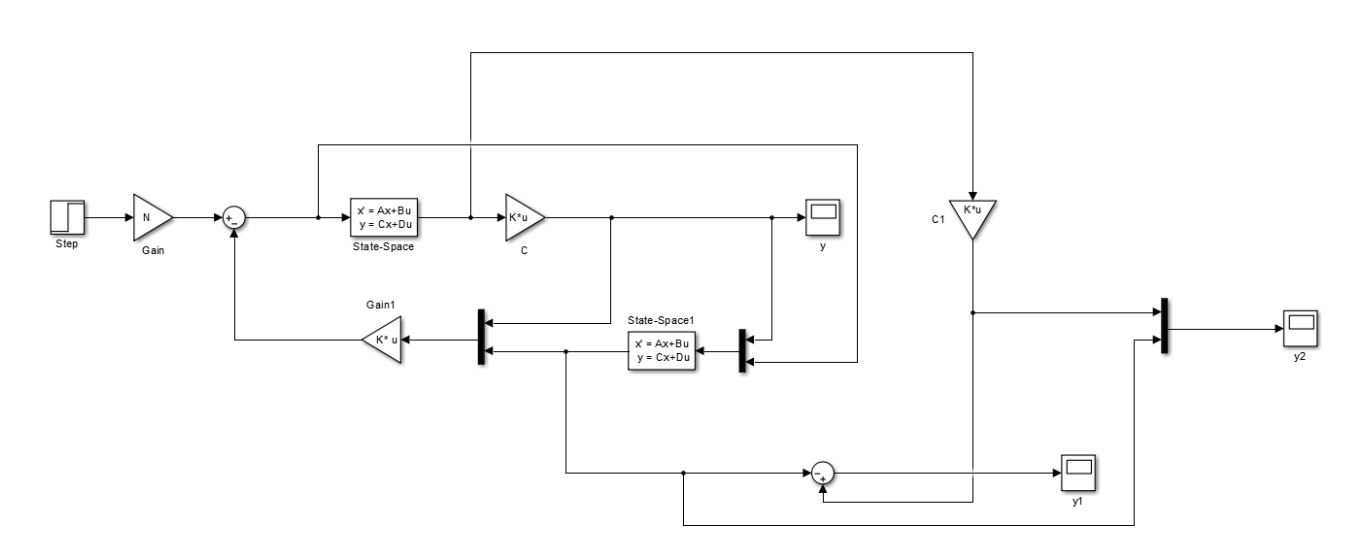
\includegraphics[scale = 0.35]{OBS_MINI.JPG}\\[0.7 cm] 
\caption{Schéma bloc de l'observateur minmal identité}
\end{figure}
\par La simulation avec des conditions initiales tel que, $v_s(0)=\pi/2~et~\dot{v_s}(0)=0$, nous obtenons en sortie de cet observateur minimal identité ceci :
\begin{figure}[h!]
\centering
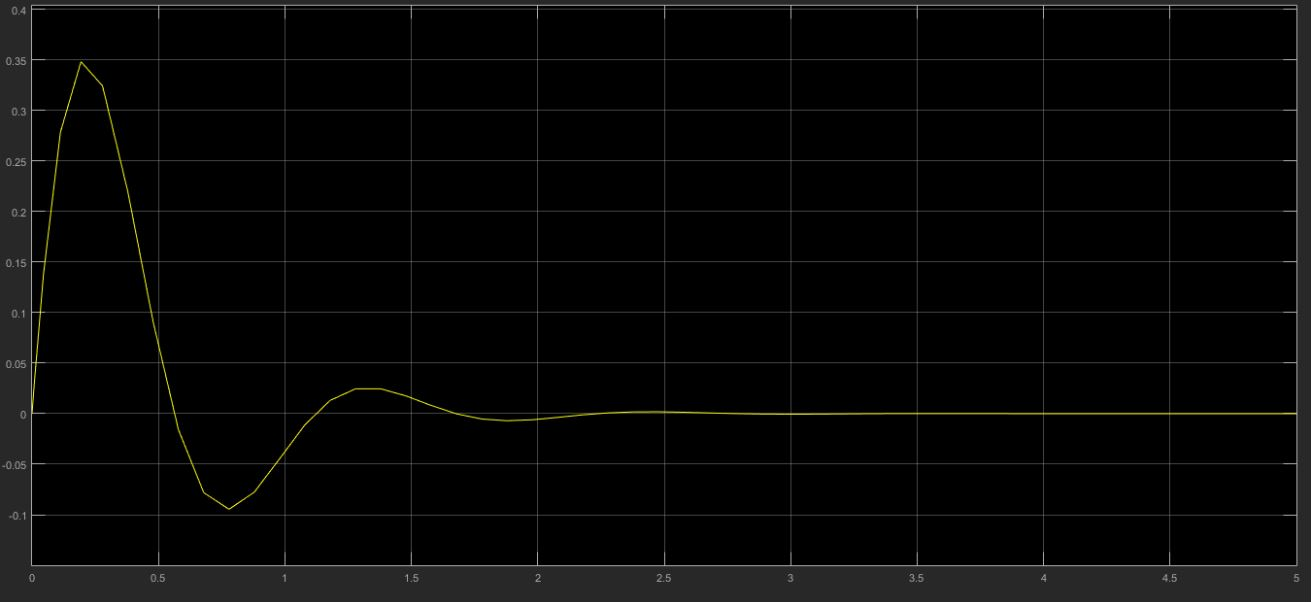
\includegraphics[scale = 0.35]{FFF1.JPG}\\[0.7 cm] 
\caption{Sortie du système avec observateur minmial identité}
\end{figure}
\par On peut conclure que le dépassement à énormément diminué comparé à l'observateur identité.


%(2)%%%%%%%%%%%%%%%%%%%%%%%%%%%%%%%%%%%%%%%%%%%%%%%%%%%%%%%%%%%%%%%%%%%%%%%%%%%%%%%%%%%%%%%%

\chapter{\textsc{Compensation par retour de sortie dynamique - observateur fonctionnel}}
\chaptermark{\textsc{Compensation par retour de sortie dynamique - observateur fonctionnel}}
\parindent=1cm 
Dans cette partie nous allons procéder à la reconstruction via un observateur fonctionnel permettant de reconstituer la valeur du retour d'état. C'est à dire un observateur qui converge vers $Kx(t)$, mais également  calculer les gains de l’observateur de manière à modifier ses valeurs propres pour que l’observateur soit 8 fois plus rapide que la dynamique de la boucle fermée. On veut donc $P_{min}=8*(-2.4)$
\par On a notre matrice A, que l'on peut écrire de cette façon :
    $$A = \begin{bmatrix}0 && 10.5820 \\0 && -3.33 \end{bmatrix}$$
\par $A_{11}=0~; A_{12}=105820~; A_{21}=0~; A_{22}=3.33$
\par Par la suite on veut résoudre ces équation : $$F_{fc}=A_{22}+T_1A_{12}$$ 
$$G_{fc} = A_{21} + T_1 A_{11} - F_{fc} T_1$$
$$ N_{fc} = k_1 - k_2T_1$$
$$H_{fc} = T  B$$
$$D'où~~~~M = k_2~~~~et~~~~T = [T_1~~1]$$
\par Il nous faut donc chercher la valeur de $T_1$. A l'aide de mathlab on utilise la fonction "acker", ce qui donne : $$T_1 = acker (A_{22}’,-A_{12}’,P_{min} ) = -1.4994$$
\par On obtient donc : $$F_{fc} = -19.2$$
\par D'où : $$G_{fc} = -287885$$
\par Puis : $$N_{fc} = 1.6006$$
\par Et : $$H_{fc} = 3.5$$
\par On peut donc écrire notre nouveau système se présentant sous cette forme :
$$A_{fc} = F_{fc}~~;~~B_{fc} = [G_{fc}~~H_{fc}]~~;
~~C_{fc} = M~~;~~D_{fc} = [N_{fc}~~0]$$

\par Nous avons par la suite modélisé le schéma bloc du système sous Simulink de cette manière :
\begin{figure}[h!]
\centering
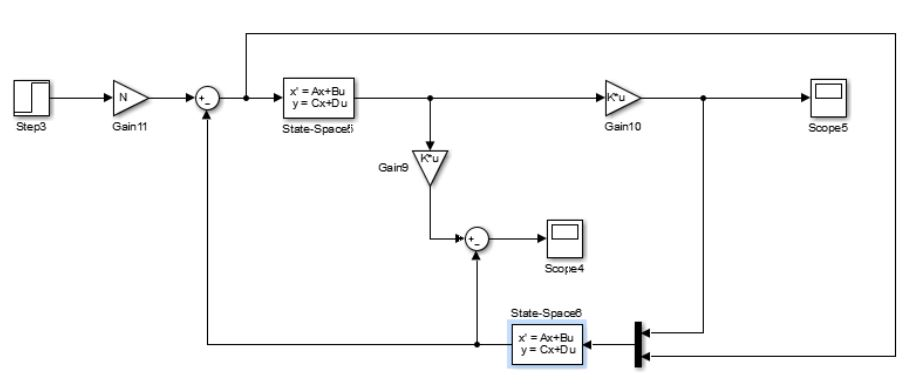
\includegraphics[scale = 0.5]{Capture.JPG}\\[0.7 cm] 
\caption{Schéma bloc observateur fonctionnel}
\end{figure}
\par La simulation avec des conditions initiales nulles ($v_s(0)=0~et~\dot{v_s}(0)=0$) nous donne un tracé comme montré ci-dessous :
\begin{figure}[h!]
\centering
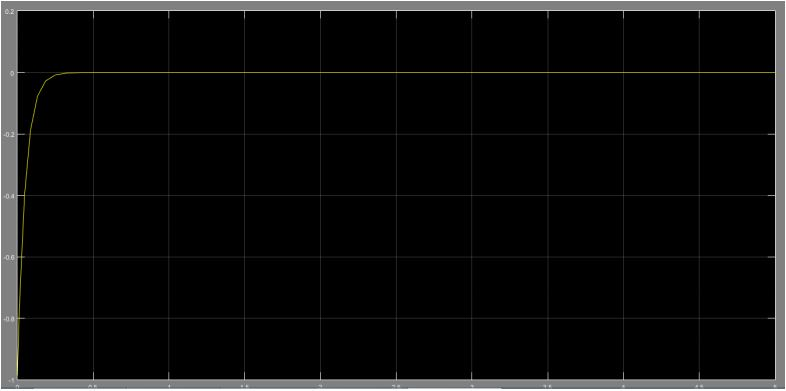
\includegraphics[scale = 0.7]{S1.JPG}\\[0.7 cm] 
\caption{Sortie du système avec observateur fonctionnel et conditions initiales nulles}
\end{figure}
\pagebreak
\par Maintenant avec des conditions initiales différentes ($v_s(0)=\pi/2~et~\dot{v_s}(0)=0$), on obtient un tracé comme montré ci-dessous :
\begin{figure}[h!]
\centering
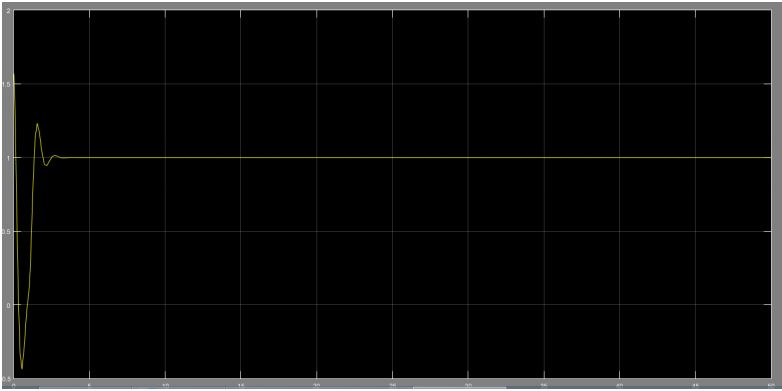
\includegraphics[scale = 0.7]{S2.JPG}\\[0.7 cm] 
\caption{Sortie du système avec observateur fonctionnel et conditions initiales différente}
\end{figure}
\par L'objectif a été atteint, car d'après le tracé on a une sortie qui est plus rapide avec le nouvel observateur fonctionnel.

%\input{conclusion.tex}

\begin{appendices}

\chapter*{\textsc{Annexe A}}
	\addcontentsline{toc}{chapter}{\textsc{Annexe A}}		
	
	Code MATLAB qui calcule la matrice de commandabilité resp(observabilité) et son rang,\label{Annexe A} \hyperref[section 1.2]{Retour vers section 1.3}
	
	\begin{lstlisting}	
clear all;
close all;
clc;

Ke = 3.6/1000*60/(2*pi);
Ks=10;
Kg=0.105;
Te = 0.01;
Km=10;
Tm=0.3;
Kc=3.5/100;

A=[0 Ks/(9*Kg);0 (-1/Tm)]
B=[0; (Km*Kg)/Tm]
C=[1 0]
D=[0]

sys=ss(A,B,C,D)

Co=ctrb(sys);
rang_co=rank(Co);

Obs=obsv(sys);
rang_obs=rank(Obs);

	\end{lstlisting}	
	
	
\chapter*{\textsc{Annexe B}}
	\addcontentsline{toc}{chapter}{\textsc{Annexe B}}		
	
	Code MATLAB qui calcule la valeur du gain matriciel K,\label{annexe B} \hyperref[K]{Retour vers section 2.2}
	\begin{lstlisting}	
	
	K=acker(A,B,[-2.4+5.5*i -2.4-5.5*i])
	
	\end{lstlisting}	
	
\chapter*{\textsc{Annexe C}}
	\addcontentsline{toc}{chapter}{\textsc{Annexe C}}		
	
	Code MATLAB qui calcule la valeur du gain N,\label{Annexe C} \hyperref[N]{Retour vers section 2.2}
	\begin{lstlisting}	
	
	Abf=A-B*K
	Bbf=B;
	Cbf=C;
	Dbf=D;
	
	sysbf=ss(Abf,Bbf,Cbf,Dbf);

	dcg=dcgain(sysbf) 
	N=1/dcg
	
	\end{lstlisting}	
	
\end{appendices}	
%*********************** Bibliographie ************ 
\bibliographystyle{alpha}
\bibliography{biblio}  



\end{document}
